\section{Architecture Review}
\label{sec:architecture_review}
In this section we review the architecture of the three services of the Basilisk platform.
We point out possible problems with current implementations and list missing implementations that need to be added.


\subsection{Code Refactoring}
\label{sec:code_refactor}
During the code analysis some inconsistencies in the code style and duplicate code snippets have been found.
In other parts the code structured differs to the design patterns recommended for the Spring and Spring Boot framework.

In general an in-depth code refactoring is recommended to increase readability and maintainability of the source code. 


\subsection{Management of Repositories and Configurations}
\label{sec:management_repo_config}
Currently the observed repositories are managed and stored in the \ac{hcs} while the configurations for the \tsp{} are managed and stored in the \ac{jms}.
This makes it difficult to internally link a repository to a \ts{} configuration, since they are stored in different services.

The current implementations tries to solve this problem, by sending events about repository creations from the \ac{hcs} to the \ac{jms}.
This results in the duplication of the repository storage in both services.
This contradicts the idea of microservice, which should be separated as much as possible from each other.

Therefore we recommend restructuring the management of repositories.


\subsection{Creation and Management of Benchmark Jobs}
\label{sec:creation_of_benchmark_jobs}
When a new release is found by the \ac{hcs}, the \acl{jms} will create and manage benchmark jobs which will be executed by the \ac{tbs}.
Currently the \ac{jms} will create multiple jobs.
For each query file a job will be created for each dataset.
This means that each dataset is mixed with each query file, which could lead to queries executed on the wrong datasets.

A benchmark should only use a defined pair of a matching query file and dataset.
Therefore the logic for creating the benchmark jobs needs to be changed, as well as the data model for storing the benchmark jobs.


\subsection{Data Model Restructure}
\label{sec:review_data_model}
The \ac{jms} manages and stores the different configuration types needed for a benchmark job.

The configurations are stored in an internal database.
Figure \ref{fig:jms_db_schema} shows the current database schema.

\begin{figure}[tbph]
	\centering
	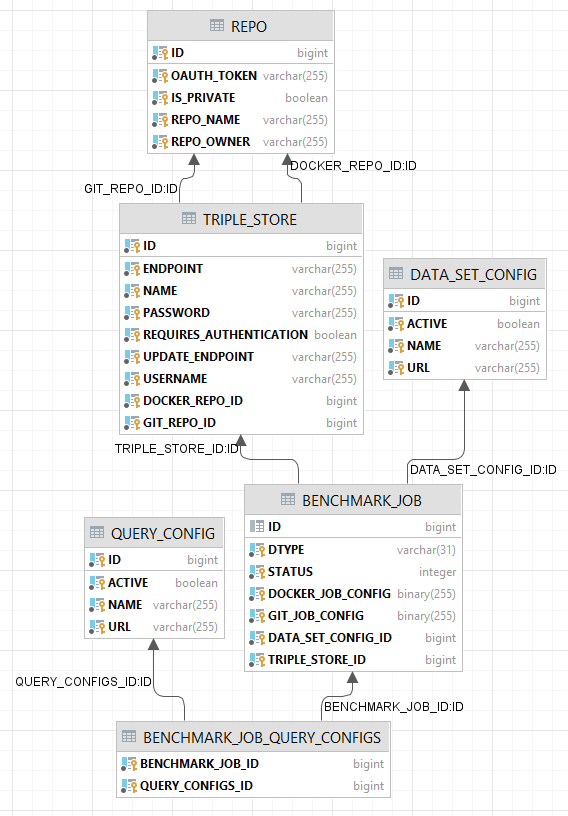
\includegraphics[width=.7\textwidth]{figures/jms_db_schema.png}
	\caption{Diagram of the current database schema used in the \ac{jms}}
	\label{fig:jms_db_schema}
\end{figure}

The schema has logical errors and is in parts incomplete.
Following we list some inconsistencies and possible problems that could arise:
\begin{itemize}
	\item The only way to identify an repository as \gh{} or \dockh{} repo is to check in the \ts{} configuration.
		If a repository is wrongly assigned to the false type, the resulting benchmark job would not be executable, because \gh{} and \dockh{} needs to be handled differently during a benchmark as explained in section \ref{sec:ts_benchmarking_service}.
	
	\item Each \ts{} configuration can have exactly one \gh{} or \dockh{} repository.
		This means for every repository a new \ts{} configuration needs to be added.
		There would be less duplicate configurations if multiple repositories could point to the same configuration.
		For example, a hook could be set up to observe a \gh{} repository for new releases and another hook could be set up to observe the same \gh{} repo for pull requests.
		In this case both hooks should use the same \ts{} configuration, since it is the same \ts{} which gets benchmarked.
		
	\item As explained in section \ref{sec:creation_of_benchmark_jobs}, the 	creation and storage of benchmark jobs needs to be changed.
		Currently the data model structure for benchmark jobs, datasets and query files is too complicated and not easy to understand.
		Since the creation process of the jobs needs to be changed, the data model will also need changes and a cleanup of the model relationships.
	
\end{itemize} 

Therefore the data model for the \ac{jms} needs a restructure to better cover real world requirements.


\subsection{Missing Implementations}
\label{sec:review_missing_impl}
The Basilisk platform is not yet fully implemented.
After reviewing the source code the following overview was created:

\subsubsection{\acl{hcs}}
The implementation of the \acl{hcs} is quite complete.
Small additions have to be implemented.

\begin{itemize}
	\item The REST endpoints for deleting \gh{} and \dockh{} repositories needs to be added.
	
	\item Currently Pull Requests for \gh{} repositories can not be observed.
\end{itemize}


\subsubsection{\acl{jms}}
The implementation of the \acl{jms} is mainly missing the REST API and some internal logic.
The following REST endpoints have to be added:

\begin{itemize}
	\item Adding / removing \ts{} configurations
	
	\item Adding / removing dataset configurations
	
	\item Adding / removing query configurations
\end{itemize}

Since the \ac{jms} also manages the running and pending benchmark jobs, the REST API and internal logic for managing these jobs needs to be implemented too.

\begin{itemize}
	\item List running / pending jobs and their status
	
	\item Set the status for a job
\end{itemize}



\subsubsection{\acl{tbs}}
The implementation of the \acl{tbs} currently contains only a few classes for the data models, and simple structures of service classes.
Big parts of the logic still needs to be implemented.

The existing classes are mainly for storing and manipulating data models, configurations and basic message queue interactions.
These classes do not carry much functionality.

The main functionality needs to be implemented.
This consists of setting up the Docker containers which contain the \tsp{} for benchmarking:

\begin{itemize}
	\item Pulling Code from \gh{}
	\item Pulling images form \dockh{}
	
	\item building Docker containers from Dockerfiles / images
	
	\item connection to the Docker containers
\end{itemize}

Then the usage of the \iguana{} framework needs to be implemented.
The framework needs to be setup to write the benchmark results to the \acl{jsts}.
\\

To have a better control of the running jobs and the benchmarking service in general we recommend to add a small REST API.
This API could be similar to the one of the \ac{hcs}, that starts and stops the continuous checking.
The API for the \ac{tbs} can function like a switch, which indicates if a new benchmarking job will be started or not.
If it is set to off, the current benchmarking job will be finished, but no new job will be started.

Lastly, after the performing of a benchmark, the cleanup of the Docker containers needs to be implemented.

\subsection{User Management and Security}
\label{sec:review_user_management}
The Basilisk platform has no user management or any kind of access control implemented.
Currently the REST APIs of the services allow interactions with any user.
If the platform is needed to run publicly, some user management and further security measures are needed.
That includes registering new users and user groups with different user rights.
Some users should only be able to read benchmark results, while other should be able to create repositories and abort jobs.

Secondly, confidential information need to be kept secret.
This is for example the OAuth-Key needed for accessing private \gh{} repositories.


\subsection{Frontend}
\label{sec:review_frontend}
The frontend introduces a new programming languages and frameworks.
A short review of the current source code resulted in the following findings:
\begin{itemize}
	\item Currently only a small web view is implemented
	\item Functionality to communicate with the REST APIs is missing
\end{itemize}


As explained in section \ref{sec:time_schedule} the priority for the frontend has been lowered.
The focus for the thesis lies in finishing the main services and their functionality.

